\documentclass[a4paper]{article}

\usepackage[a4paper, total={18cm, 26cm}]{geometry}
\usepackage[T1]{fontenc} % needed by beramono
\usepackage{textcomp}
\usepackage{textgreek} % Greek letters
% beramono.sty and MnSymbol.sty come with texlive-fonts-extra in Debian
\usepackage[scaled=0.85]{beramono} % tt font supporting slshape and zero with dot
\usepackage{MnSymbol} % fancy symbols for line-breaks
\usepackage[utf8]{inputenc}
\usepackage{listingsutf8}  % code listings, comes with texlive-latex-recommended
%\usepackage{listings}
\usepackage{xcolor}
\usepackage{verbatim}
\usepackage{graphicx} % \includegraphics[width=\textwidth]{image.png}
\usepackage{pdfpages} % insert PDF, comes with texlive-latex-recommended
\usepackage{booktabs}

% special characters: https://tex.stackexchange.com/a/574950/35131
\lstset{
  inputencoding=utf8,
  extendedchars=true,
  literate={±}{$\pm$}1 {∅}{$\emptyset$}1
      {á}{{\'a}}1  {é}{{\'e}}1  {í}{{\'i}}1 {ó}{{\'o}}1  {ú}{{\'u}}1
      {Á}{{\'A}}1  {É}{{\'E}}1  {Í}{{\'I}}1 {Ó}{{\'O}}1  {Ú}{{\'U}}1
      {à}{{\`a}}1  {è}{{\`e}}1  {ì}{{\`i}}1 {ò}{{\`o}}1  {ù}{{\`u}}1
      {À}{{\`A}}1  {È}{{\`E}}1  {Ì}{{\`I}}1 {Ò}{{\`O}}1  {Ù}{{\`U}}1
      {ä}{{\"a}}1  {ë}{{\"e}}1  {ï}{{\"i}}1 {ö}{{\"o}}1  {ü}{{\"u}}1
      {Ä}{{\"A}}1  {Ë}{{\"E}}1  {Ï}{{\"I}}1 {Ö}{{\"O}}1  {Ü}{{\"U}}1
      {â}{{\^a}}1  {ê}{{\^e}}1  {î}{{\^i}}1 {ô}{{\^o}}1  {û}{{\^u}}1
      {Â}{{\^A}}1  {Ê}{{\^E}}1  {Î}{{\^I}}1 {Ô}{{\^O}}1  {Û}{{\^U}}1
      {œ}{{\oe}}1  {Œ}{{\OE}}1  {æ}{{\ae}}1 {Æ}{{\AE}}1  {ß}{{\ss}}1
      {ẞ}{{\SS}}1  {ç}{{\c{c}}}1 {Ç}{{\c{C}}}1 {ø}{{\o}}1  {Ø}{{\O}}1
      {å}{{\aa}}1  {Å}{{\AA}}1  {ã}{{\~a}}1  {õ}{{\~o}}1 {Ã}{{\~A}}1
      {Õ}{{\~O}}1  {ñ}{{\~n}}1  {Ñ}{{\~N}}1  {¿}{{?`}}1  {¡}{{!`}}1
      {„}{\quotedblbase}1 {“}{\textquotedblleft}1 {–}{$-$}1 {-}{$-$}1
      {°}{{\textdegree}}1 {º}{{\textordmasculine}}1 {ª}{{\textordfeminine}}1
      {€}{{\EUR}}1 {£}{{\pounds}}1  {©}{{\copyright}}1  {®}{{\textregistered}}1
      {«}{{\guillemotleft}}1  {»}{{\guillemotright}}1  {Ð}{{\DH}}1  {ð}{{\dh}}1
      {Ý}{{\'Y}}1    {ý}{{\'y}}1    {Þ}{{\TH}}1    {þ}{{\th}}1    {Ă}{{\u{A}}}1
      {ă}{{\u{a}}}1  {Ą}{{\k{A}}}1  {ą}{{\k{a}}}1  {Ć}{{\'C}}1    {ć}{{\'c}}1
      {Č}{{\v{C}}}1  {č}{{\v{c}}}1  {Ď}{{\v{D}}}1  {ď}{{\v{d}}}1  {Đ}{{\DJ}}1
      {đ}{{\dj}}1    {Ė}{{\.{E}}}1  {ė}{{\.{e}}}1  {Ę}{{\k{E}}}1  {ę}{{\k{e}}}1
      {Ě}{{\v{E}}}1  {ě}{{\v{e}}}1  {Ğ}{{\u{G}}}1  {ğ}{{\u{g}}}1  {Ĩ}{{\~I}}1
      {ĩ}{{\~\i}}1   {Į}{{\k{I}}}1  {į}{{\k{i}}}1  {İ}{{\.{I}}}1  {ı}{{\i}}1
      {Ĺ}{{\'L}}1    {ĺ}{{\'l}}1    {Ľ}{{\v{L}}}1  {ľ}{{\v{l}}}1  {Ł}{{\L{}}}1
      {ł}{{\l{}}}1   {Ń}{{\'N}}1    {ń}{{\'n}}1    {Ň}{{\v{N}}}1  {ň}{{\v{n}}}1
      {Ő}{{\H{O}}}1  {ő}{{\H{o}}}1  {Ŕ}{{\'{R}}}1  {ŕ}{{\'{r}}}1  {Ř}{{\v{R}}}1
      {ř}{{\v{r}}}1  {Ś}{{\'S}}1    {ś}{{\'s}}1    {Ş}{{\c{S}}}1  {ş}{{\c{s}}}1
      {Š}{{\v{S}}}1  {š}{{\v{s}}}1  {Ť}{{\v{T}}}1  {ť}{{\v{t}}}1  {Ũ}{{\~U}}1
      {ũ}{{\~u}}1    {Ū}{{\={U}}}1  {ū}{{\={u}}}1  {Ů}{{\r{U}}}1  {ů}{{\r{u}}}1
      {Ű}{{\H{U}}}1  {ű}{{\H{u}}}1  {Ų}{{\k{U}}}1  {ų}{{\k{u}}}1  {Ź}{{\'Z}}1
      {ź}{{\'z}}1    {Ż}{{\.Z}}1    {ż}{{\.z}}1    {Ž}{{\v{Z}}}1  {ž}{{\v{z}}}1
      {α}{{\textalpha}}1   {Α}{{\textAlpha}}1
      {β}{{\textbeta}}1    {Β}{{\textBeta}}1
      {γ}{{\textgamma}}1   {Γ}{{\textGamma}}1
      {δ}{{\textdelta}}1   {Δ}{{\textDelta}}1
      {ε}{{\textepsilon}}1 {Ε}{{\textEpsilon}}1
      {ζ}{{\textzeta}}1    {Ζ}{{\textZeta}}1
      {η}{{\texteta}}1     {Η}{{\textEta}}1
      {θ}{{\texttheta}}1   {Θ}{{\textTheta}}1
      {ι}{{\textiota}}1    {Ι}{{\textIota}}1
      {κ}{{\textkappa}}1   {Κ}{{\textKappa}}1
      {λ}{{\textlambda}}1  {Λ}{{\textLambda}}1
      {μ}{{\textmugreek}}1 {Μ}{{\textMu}}1
      {ν}{{\textnu}}1      {Ν}{{\textNu}}1
      {ξ}{{\textxi}}1      {Ξ}{{\textXi}}1
      {ο}{{\textomikron}}1 {Ο}{{\textOmikron}}1
      {π}{{\textpi}}1      {Π}{{\textPi}}1
      {ρ}{{\textrho}}1     {Ρ}{{\textRho}}1
      {σ}{{\textsigma}}1   {Σ}{{\textSigma}}1   {ς}{{\textvarsigma}}1
      {τ}{{\texttau}}1     {Τ}{{\textTau}}1
      {υ}{{\textupsilon}}1 {Υ}{{\textUpsilon}}1
      {φ}{{\textphi}}1     {Φ}{{\textPhi}}1
      {χ}{{\textchi}}1     {Χ}{{\textChi}}1
      {ψ}{{\textpsi}}1     {Ψ}{{\textPsi}}1
      {ω}{{\textomega}}1   {Ω}{{\textOmega}}1
}

\lstdefinestyle{bwC++}{
  language=C++,
  morekeywords={concept,consteval,constinit,constexpr,co_await,co_return,co_yield,final,noexcept,override,requires,static_assert,thread_local,BENCHMARK,TEST_CASE,SUBCASE,SECTION,CHECK,CHECK_FALSE,CHECK_THROWS_AS,CHECK_THROWS_AS_MESSAGE,CHECK_THROWS_WITH,CHECK_THROWS_WITH_AS,CHECK_MESSAGE,REQUIRE,REQUIRE_FALSE,REQUIRE_THROWS_AS,REQUIRE_THROWS_AS_MESSAGE,REQUIRE_THROWS_WITH,REQUIRE_THROWS_WITH_AS,REQUIRE_MESSAGE},
  basicstyle=\ttfamily,
  keywordstyle=\bfseries,
  stringstyle=\slshape,
  commentstyle=\slshape,
  morecomment=[s][\bfseries\slshape]{/**}{*/},
  morecomment=[l][\bfseries\slshape]{///},
  tabsize=4,
  showstringspaces=false,
  breaklines=true, breakatwhitespace=true,
  prebreak={\hbox{\quad$\rhookswarrow$}},
  postbreak={\hbox{$\lhookrightarrow$}},
  breakindent={-8pt}, breakautoindent=false,
  numbers=left, numberstyle=\tiny,
  frameshape={RYR}{N}{N}{YYY} %frame=tb,frameround=tttt
}

\lstdefinestyle{colorC++}{
  language=C++,
  morekeywords={concept,consteval,constinit,constexpr,co_await,co_return,co_yield,final,noexcept,override,requires,static_assert,thread_local,BENCHMARK,TEST_CASE,SUBCASE,SECTION,CHECK,CHECK_THROWS_AS,CHECK_THROWS_AS_MESSAGE,CHECK_MESSAGE,REQUIRE,REQUIRE_THROWS_AS,REQUIRE_THROWS_AS_MESSAGE,REQUIRE_MESSAGE},
  basicstyle=\ttfamily,
  keywordstyle=\textcolor{blue},
  stringstyle=\slshape\textcolor{red!70!black},
  commentstyle=\slshape\textcolor{green!50!black},
  morecomment=[s][\bfseries\slshape\textcolor{green!50!black}]{/**}{*/},
  morecomment=[l][\bfseries\slshape\textcolor{green!50!black}]{///},
  tabsize=4,
  showstringspaces=false,
  breaklines=true, breakatwhitespace=true,
  prebreak={\hbox{\quad\textcolor{red}{$\rhookswarrow$}}},
  postbreak={\hbox{\textcolor{red}{$\lhookrightarrow$}}},
  breakindent={-8pt}, breakautoindent=false,
  numbers=left, numberstyle=\tiny,
  frameshape={RYR}{N}{N}{YYY} %frame=tb,frameround=tttt
}

\lstdefinelanguage{CMake}{
  keywords={add_compile_definitions,add_compile_options,add_custom_command,add_custom_target,add_executable,add_library,add_link_options,add_subdirectory,add_test,cmake_minimum_required,cmake_policy,configure_file,else,enable_testing,endif,execute_process,FetchContent_Declare,FetchContent_MakeAvailable,find_package,find_library,if,include,include_directories,install,message,option,project,set,set_tests_properties,string,target_link_libraries},
  keywords=[2]{AND,BOOL,CACHE,CMAKE_BUILD_TYPE,CMAKE_CXX_FLAGS,CMAKE_CXX_STANDARD,CMAKE_CXX_STANDARD_REQUIRED,CMAKE_CXX_EXTENSIONS,CMAKE_EXPORT_COMPILE_COMMANDS,COMMAND,COMMENT,FALSE,FETCHCONTENT_QUIET,FETCHCONTENT_UPDATES_DISCONNECTED,GIT_REPOSITORY,GIT_TAG,GIT_SHALLOW,GIT_PROGRESS,INTERFACE,NAME,NOT,OBJECT,OFF,ON,OR,OUTPUT_VARIABLE,PRIVATE,PROJECT_ROOT,PROPERTIES,PUBLIC,RUN_SERIAL,STATIC,STATUS,STRING,TRUE,USES_TERMINAL_DOWNLOAD,VERSION},
  comment=[l]{\#},
  string=[s]{"}{"}
}

\lstdefinestyle{colorCMake}{
  language=CMake,
  basicstyle=\ttfamily,
  keywordstyle=\textcolor{blue},
  keywordstyle=[2]\textcolor{red!70!black},
  stringstyle=\slshape\textcolor{red!70!black},
  commentstyle=\slshape\textcolor{green!50!black},
  morecomment=[s][\bfseries\slshape\textcolor{green!50!black}]{/**}{*/},
  tabsize=4,
  showstringspaces=false,
  breaklines=true, breakatwhitespace=true,
  prebreak={\hbox{\quad\textcolor{red}{$\rhookswarrow$}}},
  postbreak={\hbox{\textcolor{red}{$\lhookrightarrow$}}},
  breakindent={-8pt}, breakautoindent=false,
  numbers=left, numberstyle=\tiny,
  frameshape={RYR}{N}{N}{YYY} %frame=tb,frameround=tttt
}

\lstdefinestyle{colorBash}{
  language=bash,
  basicstyle=\ttfamily,
  keywordstyle=\textcolor{blue},
  stringstyle=\slshape\textcolor{red!70!black},
  commentstyle=\slshape\textcolor{green!50!black},
  morecomment=[s][\bfseries\slshape\textcolor{green!50!black}]{/**}{*/},
  tabsize=4,
  showstringspaces=false,
  breaklines=true, breakatwhitespace=true,
  prebreak={\hbox{\quad\textcolor{red}{$\rhookswarrow$}}},
  postbreak={\hbox{\textcolor{red}{$\lhookrightarrow$}}},
  breakindent={-8pt}, breakautoindent=false,
  numbers=left, numberstyle=\tiny,
  frameshape={RYR}{N}{N}{YYY} %frame=tb,frameround=tttt
}

\title{sP Exam Project}
\author{Caspar Emil Jensen, Lucas Lybek Højlund Pedersen \\Pætur Magnussen, Thomas Dam Nykjær \& Thomas Ilum Andersen}
\begin{document}
  \maketitle
  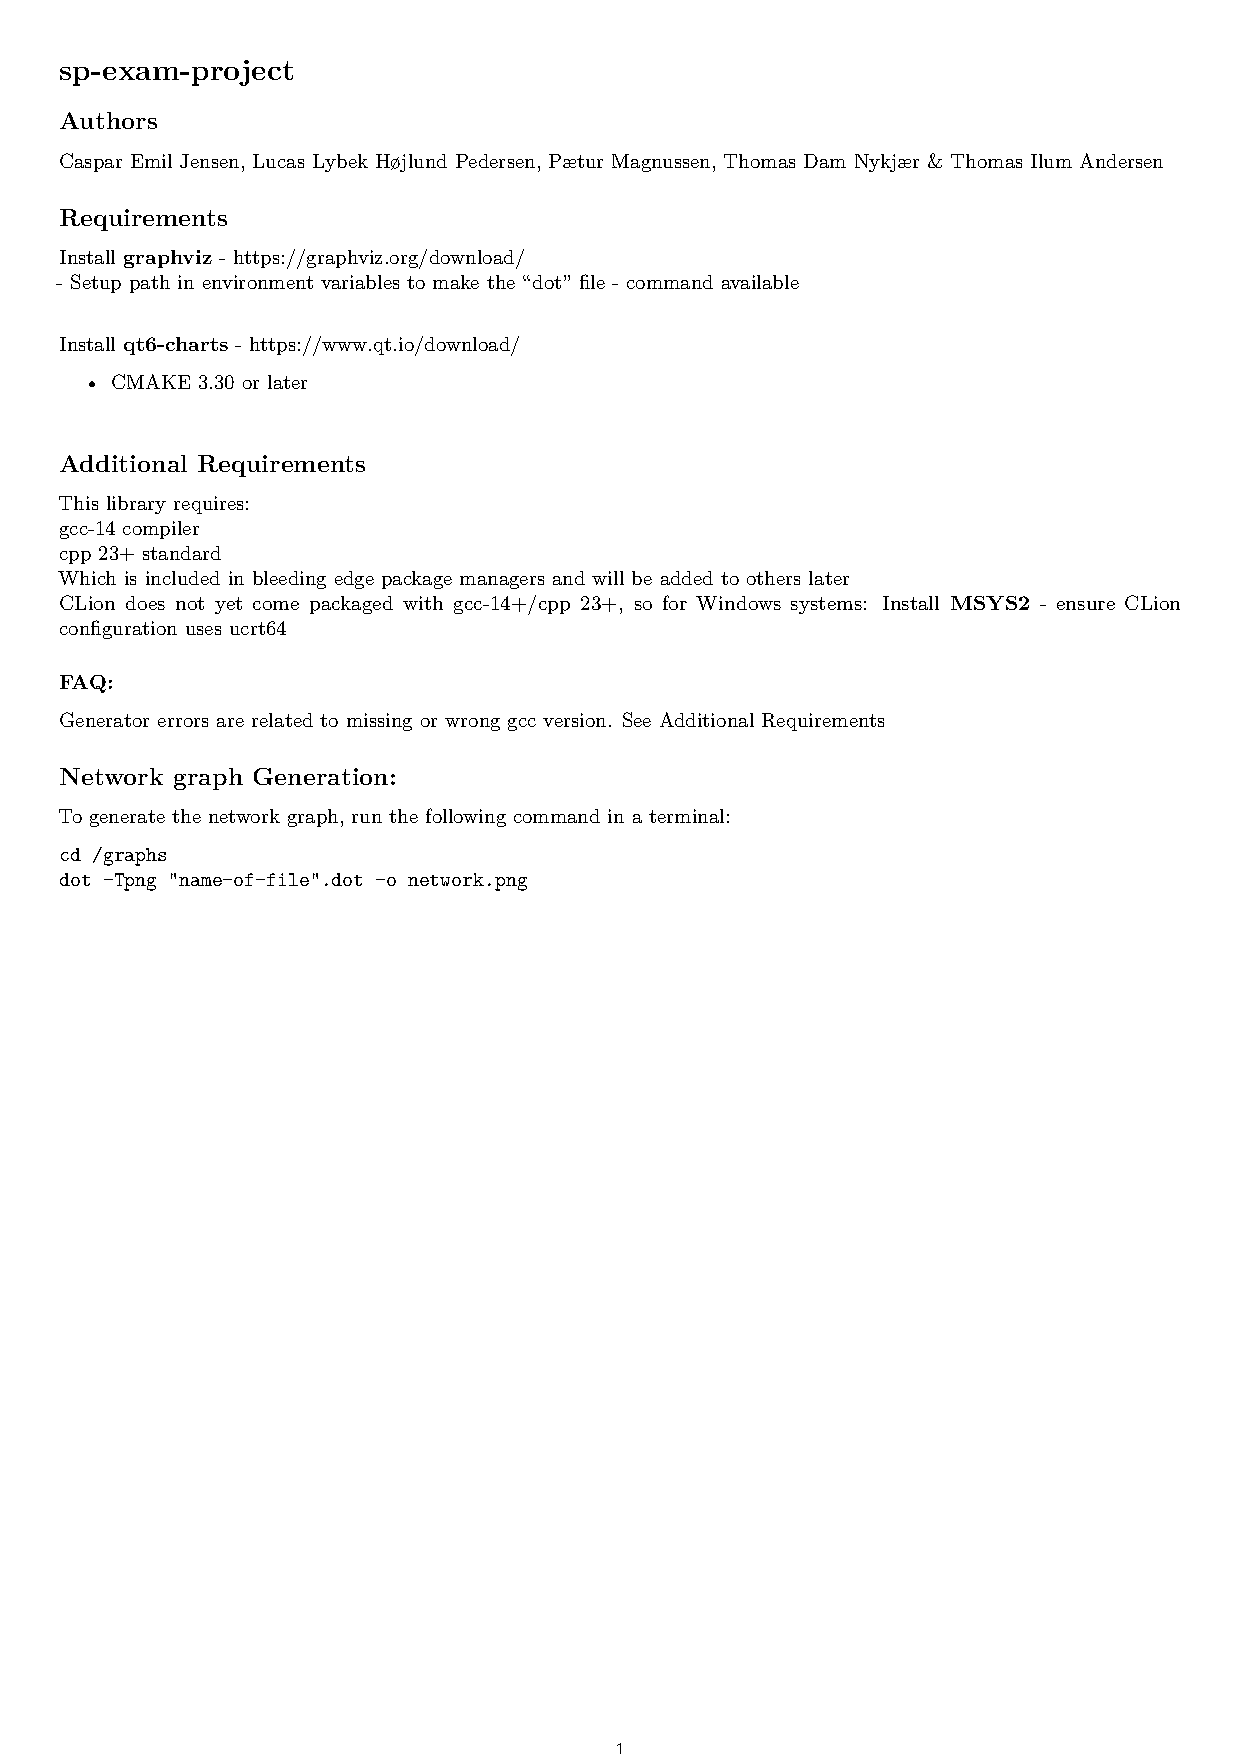
\includepdf[pages=-]{./README.md.pdf}
  % \lstinputlisting[style=colorBash,caption={Studio-log.txt}]{Studio-log.txt}
  % \lstinputlisting[style=colorBash,caption={./graphs/benchmark.txt}]{./graphs/benchmark.txt}
  % \lstinputlisting[style=colorBash,caption={./graphs/reaction.txt}]{./graphs/reaction.txt}
  \lstinputlisting[style=colorC++,caption={./bin/src/utils.hpp}]{./bin/src/utils.hpp}
  \lstinputlisting[style=colorC++,caption={./lib/examples/circadian\_rhythm.hpp}]{./lib/examples/circadian_rhythm.hpp}
  \lstinputlisting[style=colorC++,caption={./lib/examples/covid-19.hpp}]{./lib/examples/covid-19.hpp}
  \lstinputlisting[style=colorC++,caption={./lib/examples/exponential\_decay.hpp}]{./lib/examples/exponential_decay.hpp}
  \lstinputlisting[style=colorC++,caption={./lib/examples/multi\_threading.hpp}]{./lib/examples/multi_threading.hpp}
  \lstinputlisting[style=colorC++,caption={./lib/include/charter.hpp}]{./lib/include/charter.hpp}
  \lstinputlisting[style=colorC++,caption={./lib/include/debug\_print.hpp}]{./lib/include/debug_print.hpp}
  \lstinputlisting[style=colorC++,caption={./lib/include/multithreading.hpp}]{./lib/include/multithreading.hpp}
  \lstinputlisting[style=colorC++,caption={./lib/include/reaction.hpp}]{./lib/include/reaction.hpp}
  \lstinputlisting[style=colorC++,caption={./lib/include/simulator.hpp}]{./lib/include/simulator.hpp}
  \lstinputlisting[style=colorC++,caption={./lib/include/species.hpp}]{./lib/include/species.hpp}
  \lstinputlisting[style=colorC++,caption={./lib/include/state.hpp}]{./lib/include/state.hpp}
  \lstinputlisting[style=colorC++,caption={./lib/include/symbol\_table.hpp}]{./lib/include/symbol_table.hpp}
  \lstinputlisting[style=colorC++,caption={./lib/include/trajectory\_chart\_widget.hpp}]{./lib/include/trajectory_chart_widget.hpp}
  \lstinputlisting[style=colorC++,caption={./lib/include/trajectory\_logger.hpp}]{./lib/include/trajectory_logger.hpp}
  \lstinputlisting[style=colorC++,caption={./lib/include/vessels.hpp}]{./lib/include/vessels.hpp}
  \lstinputlisting[style=colorC++,caption={./benchmark/benchmarks.cpp}]{./benchmark/benchmarks.cpp}
  \lstinputlisting[style=colorC++,caption={./bin/src/main.cpp}]{./bin/src/main.cpp}
  \lstinputlisting[style=colorC++,caption={./lib/examples/circadian\_rhythm.cpp}]{./lib/examples/circadian_rhythm.cpp}
  \lstinputlisting[style=colorC++,caption={./lib/examples/covid-19.cpp}]{./lib/examples/covid-19.cpp}
  \lstinputlisting[style=colorC++,caption={./lib/examples/exponential\_decay.cpp}]{./lib/examples/exponential_decay.cpp}
  \lstinputlisting[style=colorC++,caption={./lib/examples/multi\_threading.cpp}]{./lib/examples/multi_threading.cpp}
  \lstinputlisting[style=colorC++,caption={./lib/src/charter.cpp}]{./lib/src/charter.cpp}
  \lstinputlisting[style=colorC++,caption={./lib/src/reaction.cpp}]{./lib/src/reaction.cpp}
  \lstinputlisting[style=colorC++,caption={./lib/src/simulator.cpp}]{./lib/src/simulator.cpp}
  \lstinputlisting[style=colorC++,caption={./lib/src/state.cpp}]{./lib/src/state.cpp}
  \lstinputlisting[style=colorC++,caption={./lib/src/trajectory\_chart\_widget.cpp}]{./lib/src/trajectory_chart_widget.cpp}
  \lstinputlisting[style=colorC++,caption={./test/reaction\_test.cpp}]{./test/reaction_test.cpp}
  \lstinputlisting[style=colorC++,caption={./test/symbol\_table\_test.cpp}]{./test/symbol_table_test.cpp}
  \lstinputlisting[style=colorCMake,caption={./benchmark/CMakeLists.txt}]{./benchmark/CMakeLists.txt}
  \lstinputlisting[style=colorCMake,caption={./bin/src/CMakeLists.txt}]{./bin/src/CMakeLists.txt}
  \lstinputlisting[style=colorCMake,caption={./cmake/benchmark.cmake}]{./cmake/benchmark.cmake}
  \lstinputlisting[style=colorCMake,caption={./cmake/clang-format.cmake}]{./cmake/clang-format.cmake}
  \lstinputlisting[style=colorCMake,caption={./cmake/doctest.cmake}]{./cmake/doctest.cmake}
  \lstinputlisting[style=colorCMake,caption={./cmake/sanitizers.cmake}]{./cmake/sanitizers.cmake}
  \lstinputlisting[style=colorCMake,caption={./CMakeLists.txt}]{./CMakeLists.txt}
  \lstinputlisting[style=colorCMake,caption={./lib/include/CMakeLists.txt}]{./lib/include/CMakeLists.txt}
  \lstinputlisting[style=colorCMake,caption={./lib/src/CMakeLists.txt}]{./lib/src/CMakeLists.txt}
  \lstinputlisting[style=colorCMake,caption={./test/CMakeLists.txt}]{./test/CMakeLists.txt}
  

  \newpage

\noindent\large\textbf{Benchmark Results}
  \begin{table}[ht]
    \centering
    \caption{Benchmark results for 50 iterations and 100 runs (Processor: AMD Ryzen 9 5950X 16-Core)}
    \begin{tabular}{lcccc}
        \toprule
        \textbf{Benchmark} & \textbf{Time (ms)} & \textbf{CPU (ms)} & \textbf{Iterations} & \textbf{endTime} \\
        \midrule
        seihr\_single\_core & 6936    & 6910   & 50 & 100 \\
        seihr\_multi\_core & 976      & 4.69   & 50 & 100 \\
        circadian\_rhythm\_single\_core\_100\_runs & 24519 & 24432  & 50 & 48 \\
        circadian\_rhythm\_single\_core\_100\_runs\_optimized & 24512 & 24421  & 50 & 48 \\
        circadian\_rhythm\_multi\_core\_100\_runs & 4383 & 14.1   & 50 & 48 \\
        exponential\_decay\_single\_core & 8.77 & 8.75  & 50 & 1500 \\
        exponential\_decay\_multi\_core  & 8.07 & 5.00  & 50 & 1500 \\
        \bottomrule
    \end{tabular}
\end{table}

\vspace{2em}  

\noindent\large\textbf{Pretty printing of reactions}
\begin{verbatim}

  Circadian Rhythm:
  A + DA  >>  (1.00)  >>= D_A
  D_A     >> (50.00)  >>= DA + A
  A + DR  >>  (1.00)  >>= D_R
  D_R     >> (100.00) >>= DR + A
  D_A     >> (500.00) >>= MA + D_A
  DA      >> (50.00)  >>= MA + DA
  D_R     >> (50.00)  >>= MR + D_R
  DR      >>  (0.01)  >>= MR + DR
  MA      >> (50.00)  >>= MA + A
  MR      >>  (5.00)  >>= MR + R
  A + R   >>  (2.00)  >>= C
  C       >>  (1.00)  >>= R
  A       >>  (1.00)  >>= env
  R       >>  (0.20)  >>= env
  MA      >> (10.00)  >>= env
  MR      >>  (0.50)  >>= env
\end{verbatim}

  
  \begin{figure}[!htb]
    \centering
    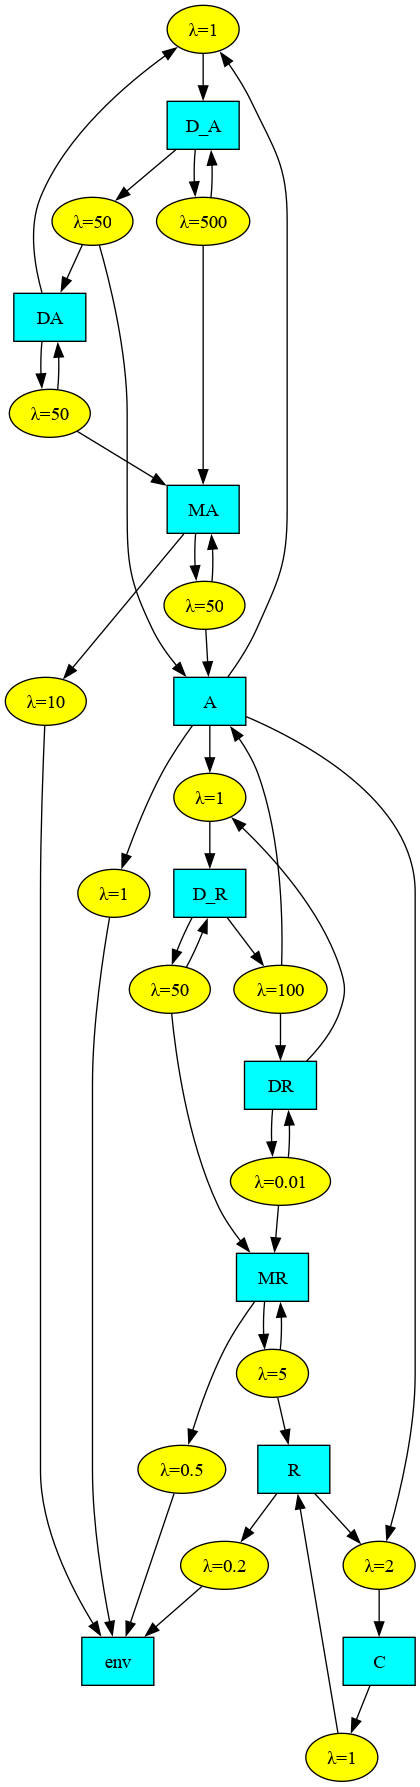
\includegraphics[height=0.95\textheight]{./graphs/circadian_rhythm.png}
    \caption{./graphs/circadian\_rhythm.png}
  \end{figure}
  \begin{figure}[!htb]
    \centering
    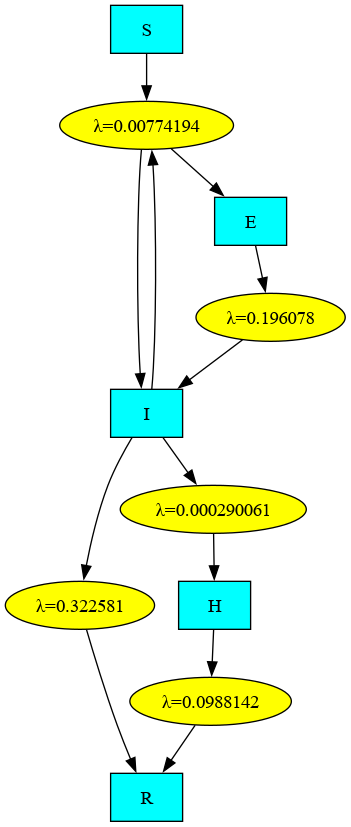
\includegraphics[height=0.95\textheight]{./graphs/covid.png}
    \caption{./graphs/covid.png}
  \end{figure}
  \begin{figure}[!htb]
    \centering
    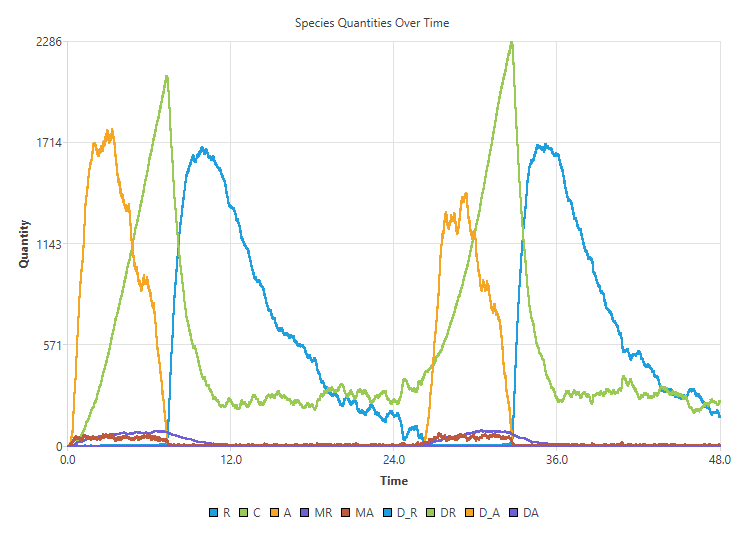
\includegraphics[width=0.95\textwidth]{./graphs/circadian.png}
    \caption{./graphs/circadian.png}
  \end{figure}
  \begin{figure}[!htb]
    \centering
    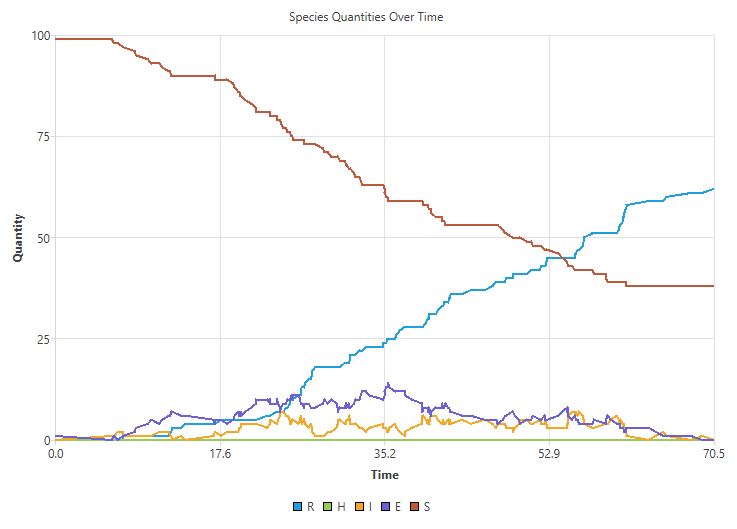
\includegraphics[width=0.95\textwidth]{./graphs/covid_sim.png}
    \caption{./graphs/covid\_sim.png}
  \end{figure}
  \begin{figure}[!htb]
    \centering
    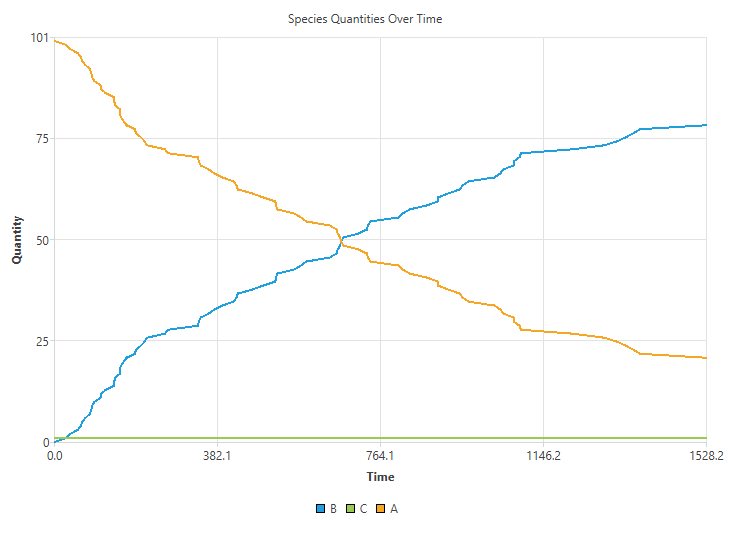
\includegraphics[width=0.95\textwidth]{./graphs/exp_dec_a.png}
    \caption{./graphs/exp\_dec\_a.png}
  \end{figure}
  \begin{figure}[!htb]
    \centering
    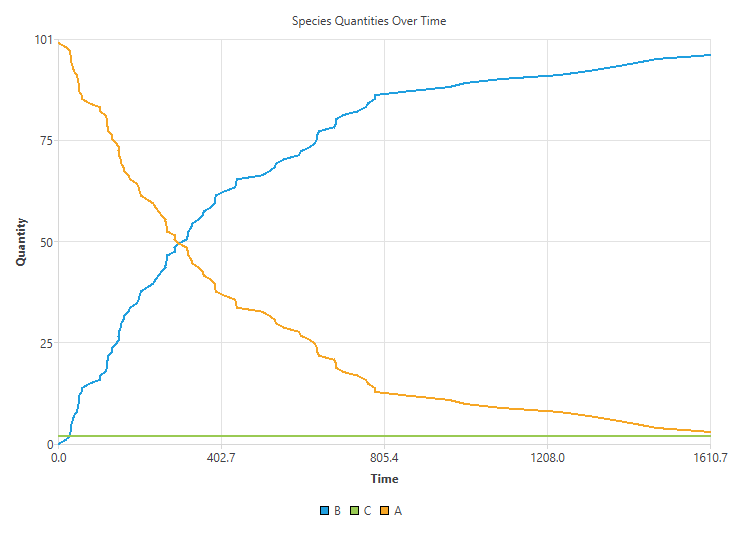
\includegraphics[width=0.95\textwidth]{./graphs/exp_dec_b.png}
    \caption{./graphs/exp\_dec\_b.png}
  \end{figure}
  \begin{figure}[!htb]
    \centering
    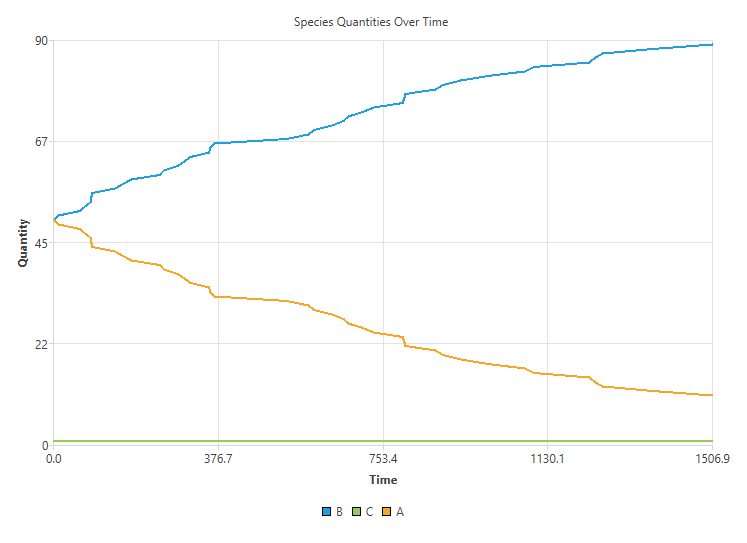
\includegraphics[width=0.95\textwidth]{./graphs/exp_dec_c.png}
    \caption{./graphs/exp\_dec\_c.png}
  \end{figure}
\end{document}
